\vspace{-0.3cm}
\section{Algorithms for Few-Shot Object Detection}

In this section, we first focus on the few-shot object detection setting. Then, we will show our two-stage fine-tuning approach in
Section~\ref{sec:tfa} and Section~\ref{sec:meta}.

% \minisection{Few-shot object detection preliminaries.}
According to~\citet{kang2019few}, We first adjust the few-shot object detection settings. We use a set of base
classes $C_b$ that have many instances and a set of novel classes $C_n$ that
have only $K$ (usually less than 10) instances per category.
For an object detection dataset $\mathcal{D}=\{(x, y), x\in\mathcal{X}, y\in\mathcal{Y}\}$ ($x$
is the input image, $y=\{(c_i, \vec{l}_i), i=1, ...,N\}$ denotes the categories $c \in C_b \cup C_n$
and bounding box coordinates $\vec{l}$ of the $N$ object instances in the image $x$).
% $y=\{(c^i, x_1^i, x_2^i, y_1^i, y_2^i), i=1, ...,N\}$

For COCO, we balcance the novel set and each class from it has the same number of 
annotated objects (\textit{i.e.}, $K$-shot). 

For LVIS, it has a natural long-tail distribution, which does
not have the manual $K$-shot split. To solve this problem, we divide the classes in LVIS into three classes, \emph{frequent} classes
(appearing in more than 100 images), \emph{common} classes (10-100 images), and \emph{rare}
classes (less than 10 images).

We evaluate our few-shot object detector on a test set with the base classes as well as
the novel classes. The goal is to optimize the detection accuracy measured by average precision (AP)
of the novel classes as well as the base classes.

\subsection{Two-stage fine-tuning approach}
\label{sec:tfa}
Our fine-tuning approach (\model) including two stages. The base detection model is formed by Faster R-CNN~\cite{ren2015faster} and a two-stage object
detector. 

As shown in Figure~\ref{fig:tfa_arch}, the feature learning components ($\mathcal{F}$) of a Faster R-CNN model include the backbone (\textit{e.g.}, ResNet~\cite{he2016deep}, VGG16~\cite{simonyan2014very}), the region proposal network (RPN), as well as a two-layer
fully-connected (FC) sub-network as a proposal-level feature extractor. 
There is also a box predictor composed of a box classifier $\mathcal{C}$ to classify the
object categories and a box regressor $\mathcal{R}$ to predict the bounding box coordinates. 
Intuitively, the backbone features as well as the RPN features
are class-agnostic. Therefore, features learned from the base classes are likely to transfer
to the novel classes without further parameter updates. The key component of our method is to separate the
feature representation learning and the box predictor learning into two stages. 

\minisection{Base model training.} This stage we use a large number of basic data samples to train ordinary 2D target detection networks (\textit{e.g.}, Faster-RCNN). This stage is the traditional training method. The loss of the network consists of three parts, 
\begin{equation}
    \mathcal{L} = \mathcal{L}_{\text{rpn}} + \mathcal{L}_{\text{cls}} + \mathcal{L}_{\text{loc}},
    \label{eq:loss}
\end{equation}
$\mathcal{L}_\text{rpn}$: the output of the RPN network. (to distinguish foreground from backgrounds and refine the
anchors)\\
$\mathcal{L}_\text{cls}$: a cross-entropy loss for the box classifier $\mathcal{C}$.\\
$\mathcal{L}_\text{loc}$: a smoothed $L_1$ loss for the box regressor $\mathcal{R}$.

\minisection{Few-shot fine-tuning.} The second stage is fine-tuning based on a small sample. While keeping the entire feature extractor unchanged, assign the randomly initialized weights of the new class to the box prediction network, and only fine-tune the box classification and regression network, which is the last layer of the detection model. This process uses the same loss function (in Equation~\ref{eq:loss}) as the first stage and reduces the learning rate. The learning rate is reduced by 20 from the first stage in all our experiments. 

\begin{figure*}[ht]
    \centering
    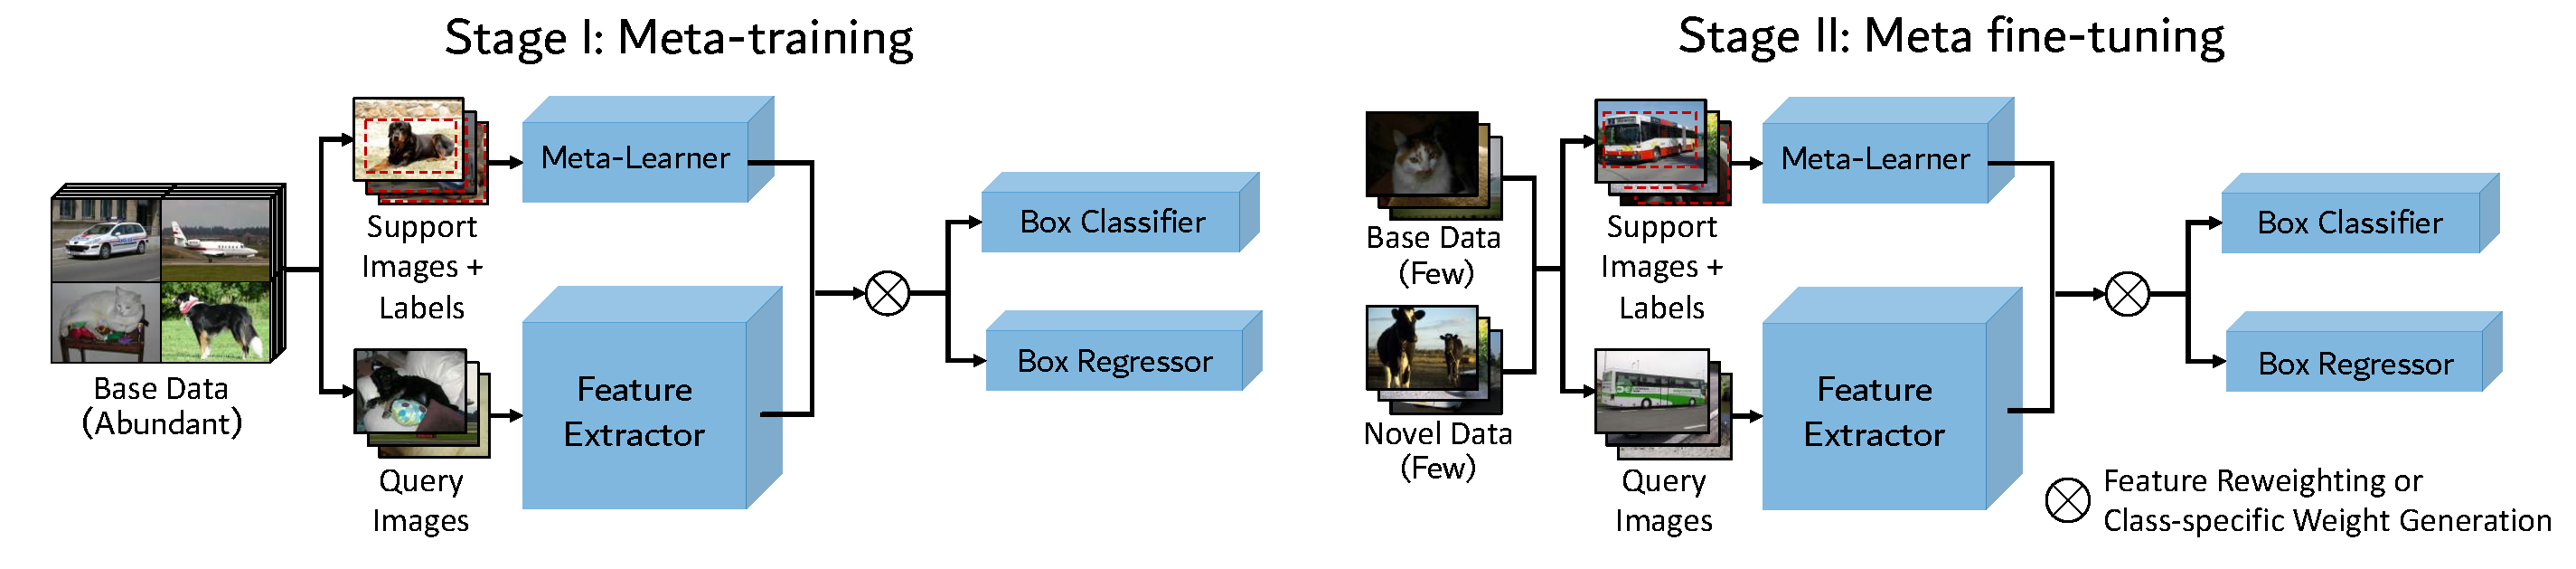
\includegraphics[width=\linewidth]{figs/TFA_fig2.pdf}
    \vspace{-8mm}
    \caption{Abstraction of the meta-learning based few-shot object detectors. A meta-learner is introduced to acquire task-level meta information and help the model generalize to novel classes through feature re-weighting (\textit{e.g.}, FSRW and Meta R-CNN) or weight generation (\textit{e.g.}, MetaDet). A two-stage training approach (meta-training and meta fine-tuning) with episodic learning is commonly adopted.}
    \label{fig:meta_arch}
\end{figure*}

\minisection{Cosine similarity for box classifier.} The design of the classifier is based on the cosine similarity function, and the formula is shown in in Equation~\ref{eq:classifier}, inspired by ~\citet{gidaris2018dynamic,qi2018low,chen2019closer}. 
The weight matrix $W\in\mathbb{R}^{d\times c}$ of the box classifier $\mathcal{C}$ can be written as $[w_1, w_2, ..., w_c]$, where $w_c\in\mathbb{R}^d$ is the per-class weight vector. The output of $\mathcal{C}$ is scaled similarity scores $S$ of the input feature $\mathcal{F}(x)$ and the weight vectors of different classes. The entries in $S$ are 
\begin{equation}
    s_{i,j} = \frac{\alpha \mathcal{F}(x)_i^\top w_j}{\|\mathcal{F}(x)_i\| \|w_j\|},
    \label{eq:classifier} 
\end{equation}
where $s_{i,j}$ is the similarity score between the $i$-th object proposal of the input $x$ and the weight vector of class $j$. $\alpha$ is the scaling factor. We use a fixed $\alpha$ of 20 in our experiments.
Compared with the FC-based classifier, the cosine similarity classifier based on instance-level feature normalization can help reduce the variance of the novel class, improve detection accuracy, especially in When the number of training samples is small.

\subsection{Compared Meta-learning based approaches with Fine-tuning approach}
\label{sec:meta}
Both the meta-learning approaches and our approach have a two-stage 
training scheme. However, we find that the episodic learning used in meta-learning approaches 
can be very memory inefficient as the number of classes when the supporting set increases. Since our
fine-tuning method only fine-tunes the last layers of the network with a normal batch training scheme, which is much more memory efficient. 
